% Chapter 4

\chapter{Method} % Main chapter title

\label{Method} % For referencing the chapter elsewhere, use \ref{Chapter1} 

\lhead{Chapter 4. \emph{Method}} % This is for the header on each page - perhaps a shortened title

In this chapter, an introduction to the problem specifications this thesis is concerning about, as well as, comprehensive documentation about the methods used, are given.


\section{Problem Introduction}

Recent work in evolutionary robotics shows that evolving the morphologies of soft robotics is possible through compositional pattern producing networks coupled with NEAT evolutionary algorithm. VoxCad simulator provides a test-bench for analyzing soft robot bodies that can be actuated through environmental changes, in this case the temperature. In addition to that, recent work by~\cite{cheney2013unshackling}, shows that very interesting morphologies can be evolved by the CPPN-NEAT algorithm in this kind of soft-robot simulation environment.

\paragraph*{VoxCad}~\\
As far as the simulation settings are concerned, it is not of interest for this thesis to explore the best  not only environmental but also material settings for the evolved soft-robots. For the simulation of the soft material bodies, VoxCad's underlying physics engine \emph{Voxelyze} was used as a stand-alone software to analyze the soft structures without rendering them. Table~\ref{VoxelyzeSimulationSettings}, describes and presents the values used in different variables of the simulation.



\paragraph*{Materials}~\\

\begin{figure}
\centering
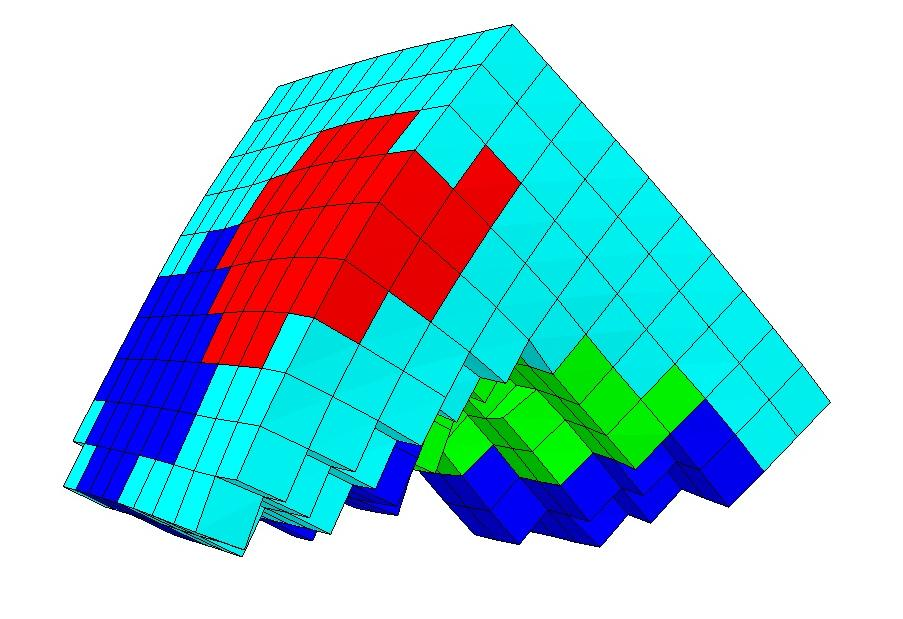
\includegraphics[height=0.2\textheight]{../Figures/Misc/allSoftMaterials.png}
\caption{Soft robot uses four materials (two active, two passive), morphology evolved penalizing actuated materials.}
\label{fig:allSoftMaterials}
\end{figure}

Figure~\ref{fig:allSoftMaterials}, illustrates a soft robot consisting of all four materials used in the experiments. \textcolor{Red}{Red} and \textcolor{Green}{Green} are the only actuated materials with non-zero and opposite thermal expansion coefficients, meaning that their phase in respect to the actuation from temperature changes is equal to half a circle, green voxels contract the same time red expand and vice versa, mimicking living organisms' muscle tissue. The two additional materials represent soft non-actuated tissue that can be soft (soft tissue) or hard (bones). \textcolor{Cyan}{Cyan} voxels are soft, having five times smaller elastic modulus of their material than \textcolor{Blue}{Blue} which have $50$ \texttt{MPa}.


\section{Direct-Generative Random Soft-Robots}
To evaluate all the following methods, information about the performance of random generated morphologies must be present. In order to achieve that, two random approaches which will also help the understanding between direct and indirect coding implemented. Direct coding which is a straightforward encoding scheme assigns randomly the presence of a voxel in a lattice's coordinate, if a voxel will be created then it will be assigned a random material from the palette. The probability of adding a voxel is $0.5$, after all voxels have been assigned a material, unconnected parts of of the structure will be removed, keeping only the largest connected structure in the lattice.


\begin{figure}
\centering
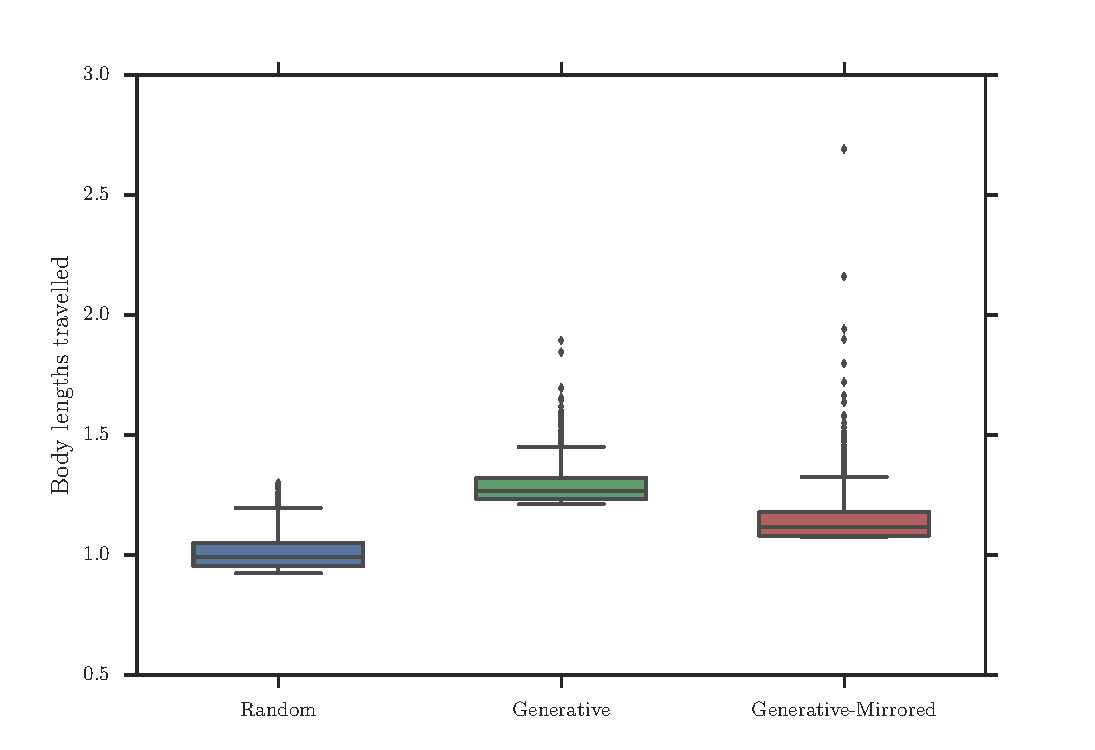
\includegraphics[width=1.0\textwidth]{../Figures/Results/random.pdf}\\
\hspace{0.1cm}
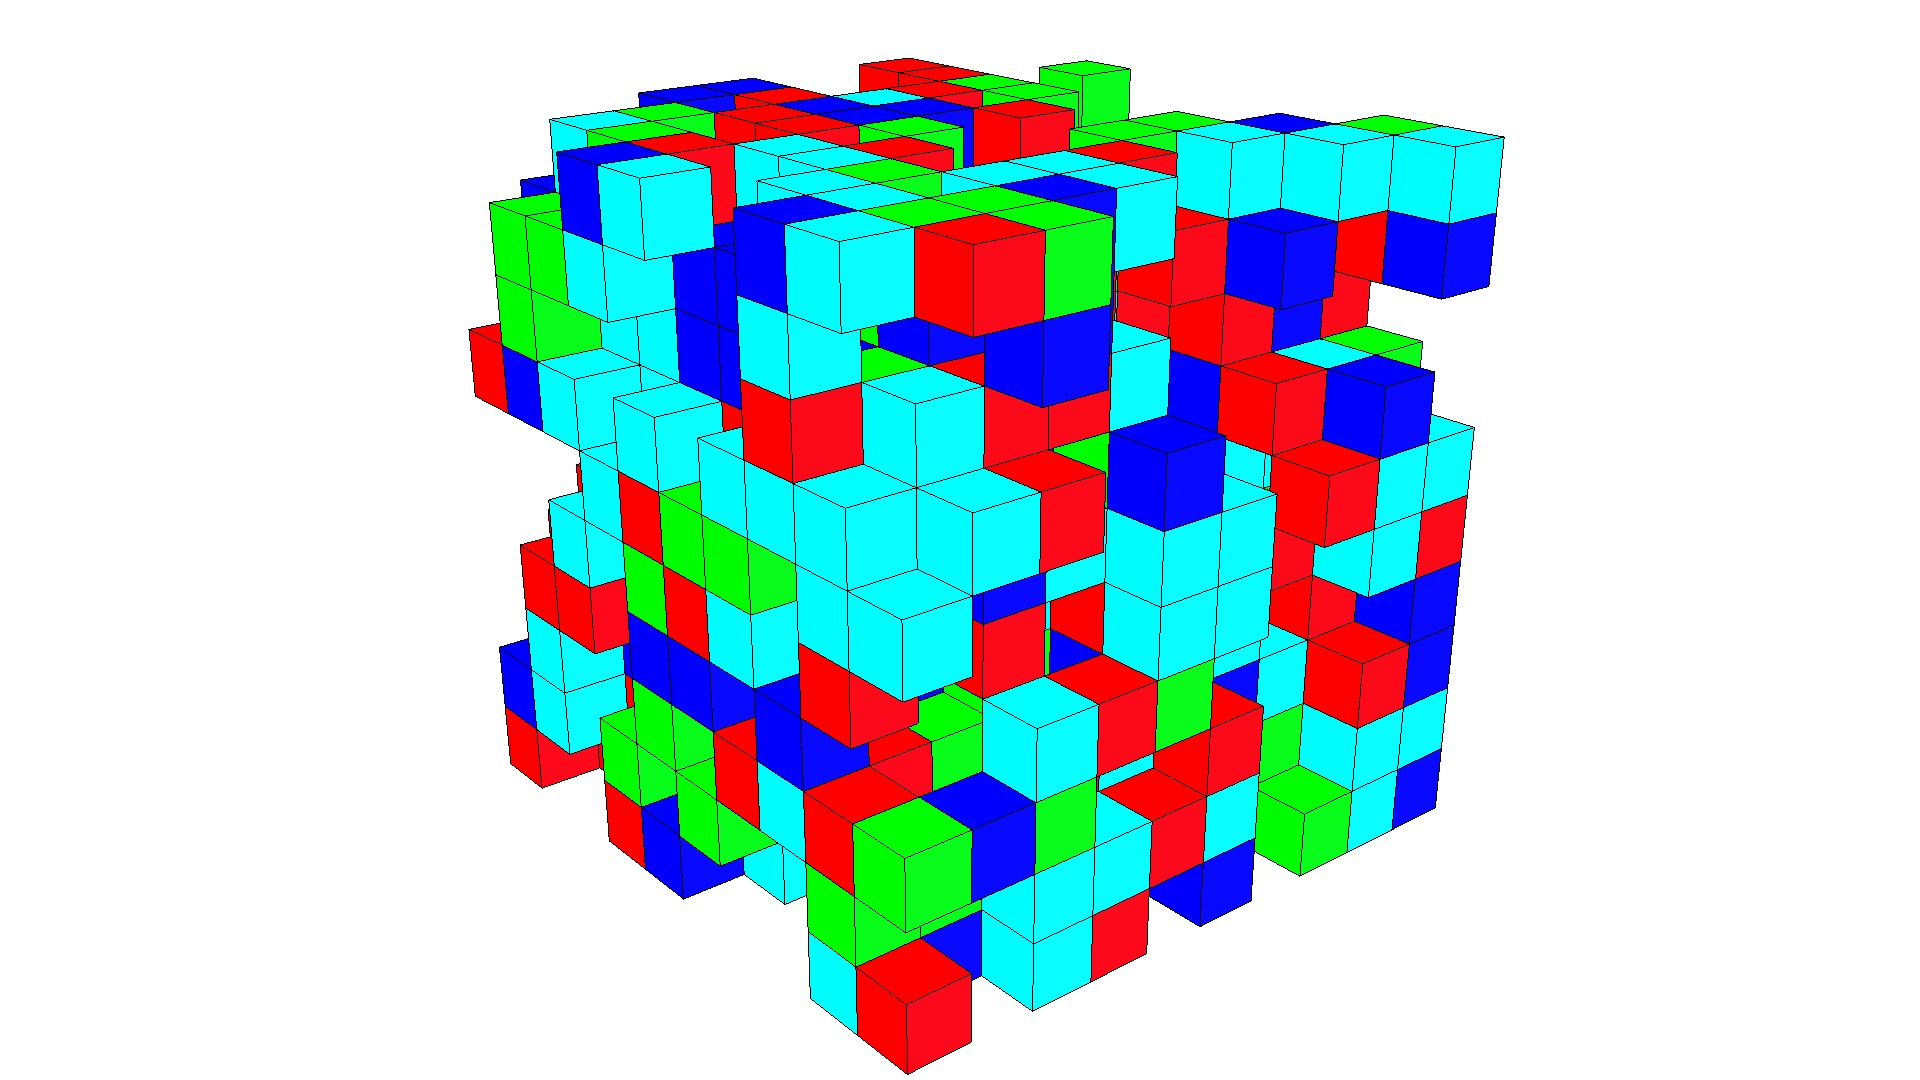
\includegraphics[height=0.15\textwidth]{../Figures/Robots/random.jpg}
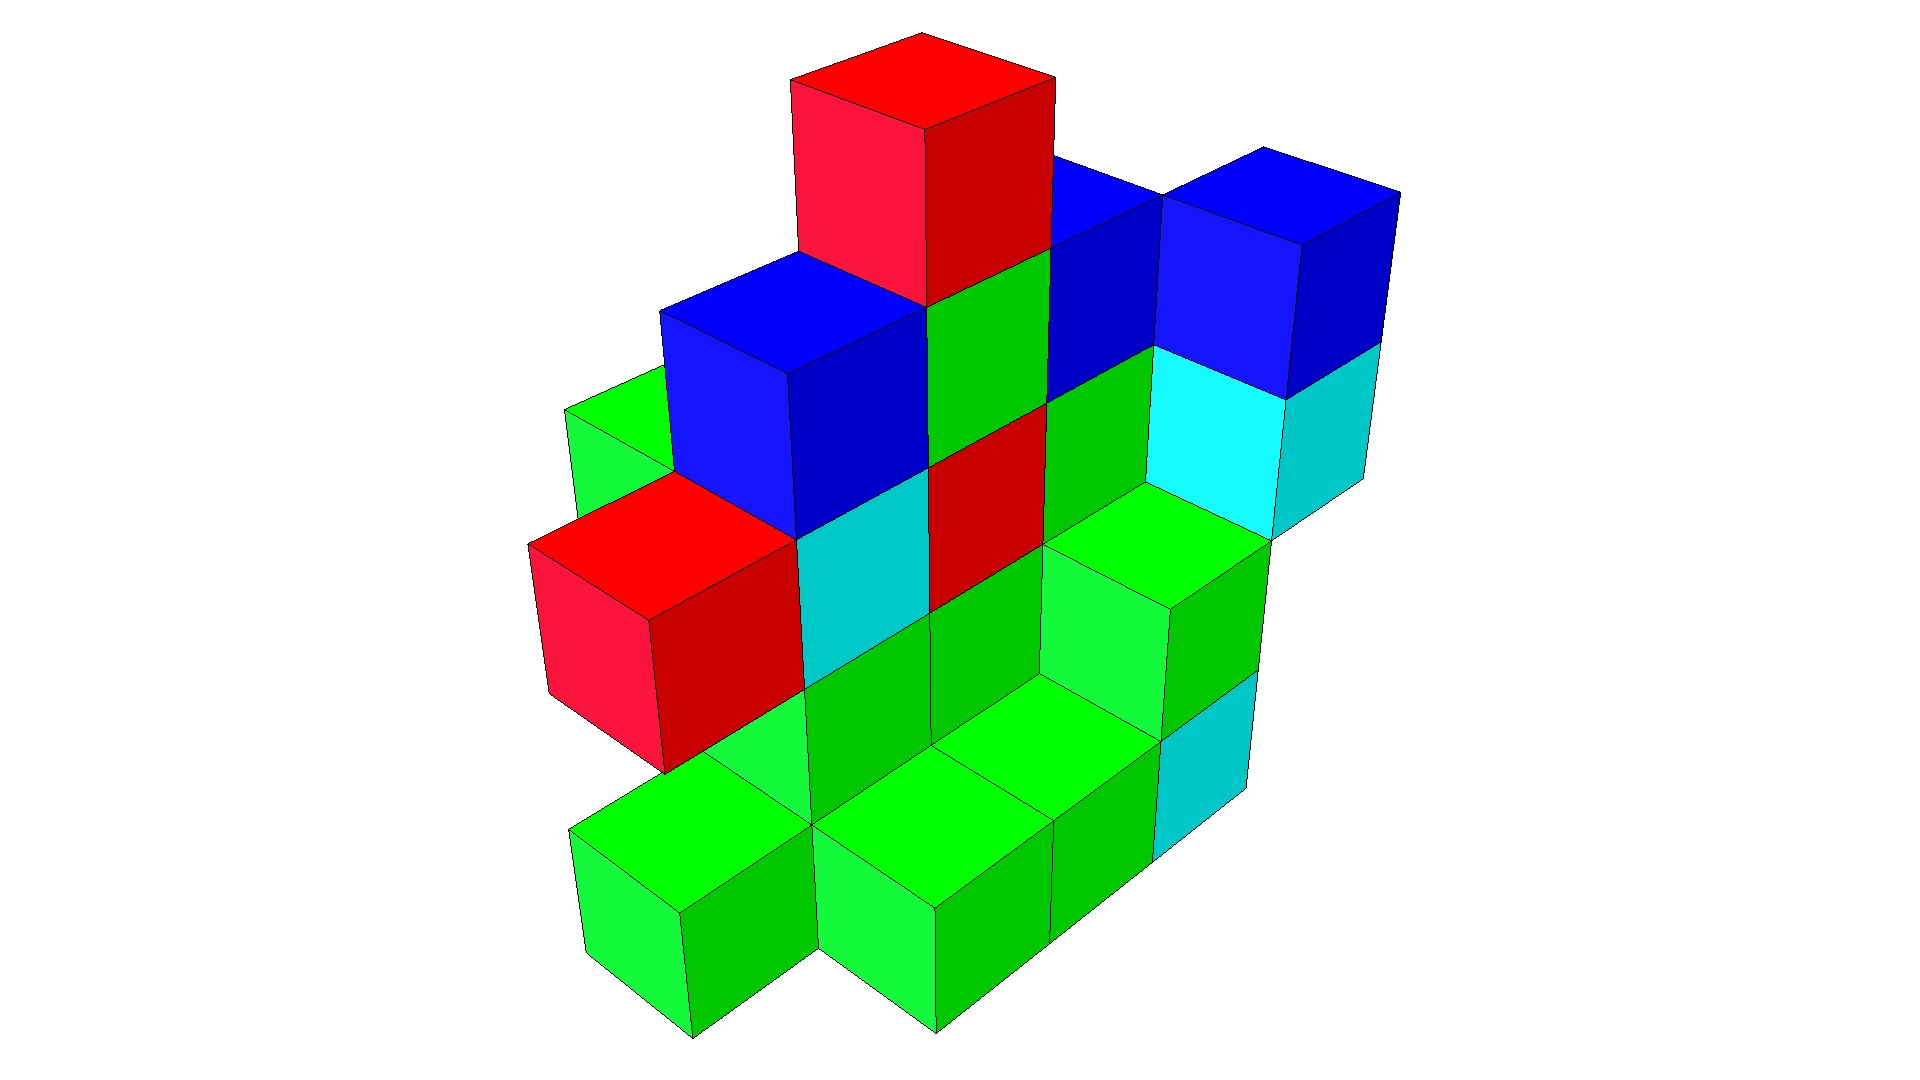
\includegraphics[height=0.15\textwidth]{../Figures/Robots/rg0.jpg}
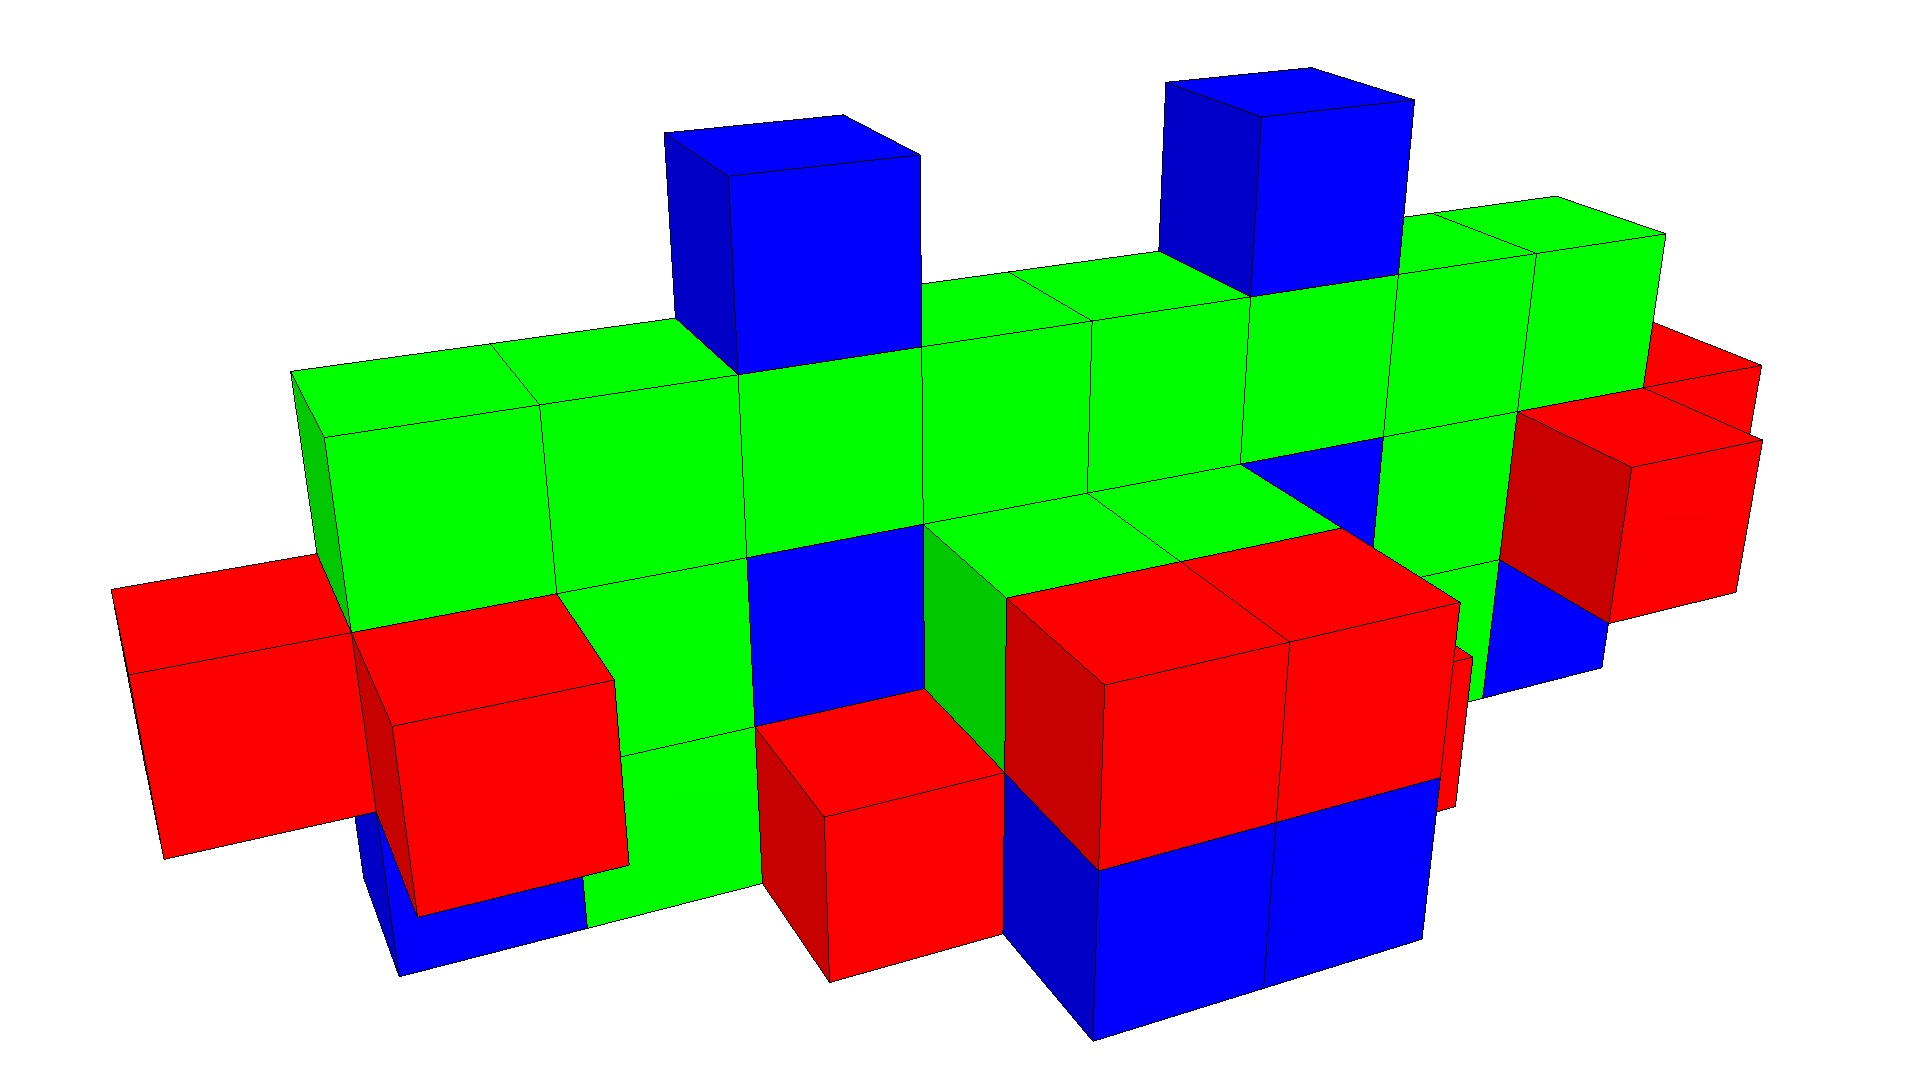
\includegraphics[height=0.15\textwidth]{../Figures/Robots/rg1.jpg}
\caption{Generative encoding creates more natural morphologies even in random schemes.}
\label{fig:randomResultsRobots}
\end{figure}


The indirect random morphology generation follows a different method of assigning materials to voxels. This methods holds two probabilities, the one refers to the probability of adding a new voxel in the already made structure, the next one denotes the probability of the new inserted material will be the same as its connection's material. First, a voxel of random material is inserted in a random coordinate into the lattice. If a new voxel is to be added a connection (voxel) is chosen from the already inserted ones. The side of the connection is chosen randomly as well, although the material itself is most of the times the same as it connected voxel's material. In this generative process there is also the possibility of creating structures in half of the lattice space, and then mirror the soft structures in both halves.

Considering these two methods, the difference between direct and indirect coding is becoming easier interpreted. In the direct process, a probability determines the presence and the material of every voxel in the lattice. On the other hand, in the generative method a set of rules and probabilities define the structure that is going to be produced into the available space.

Figure~\ref{fig:randomResultsRobots}, illustrates not only the actual performance (top-$1000$ soft-robots from $30000$ total runs for each method) of the previously described method but also one of the best performing robots of each method. Both generative methods outperform the direct one, mostly because there is no structure in the created creatures, another one reason is that since there are no rules in the construction of the random structures resulting in morphologies with huge number of voxels, something that makes them difficult to locomote. On the other hand, generative random methods create more compact structures which can move easier due to their size and some of their geometrical features. For the mirrored approach even though the average performance is slightly worse than the plain method it actually performs way better in some distinct cases. Inserting some geometrical properties like properties resulted in getting more successful locomotive structures. 

\section{Direct-Encoded Evolutionary Soft-Robots}

\begin{figure}
\centering
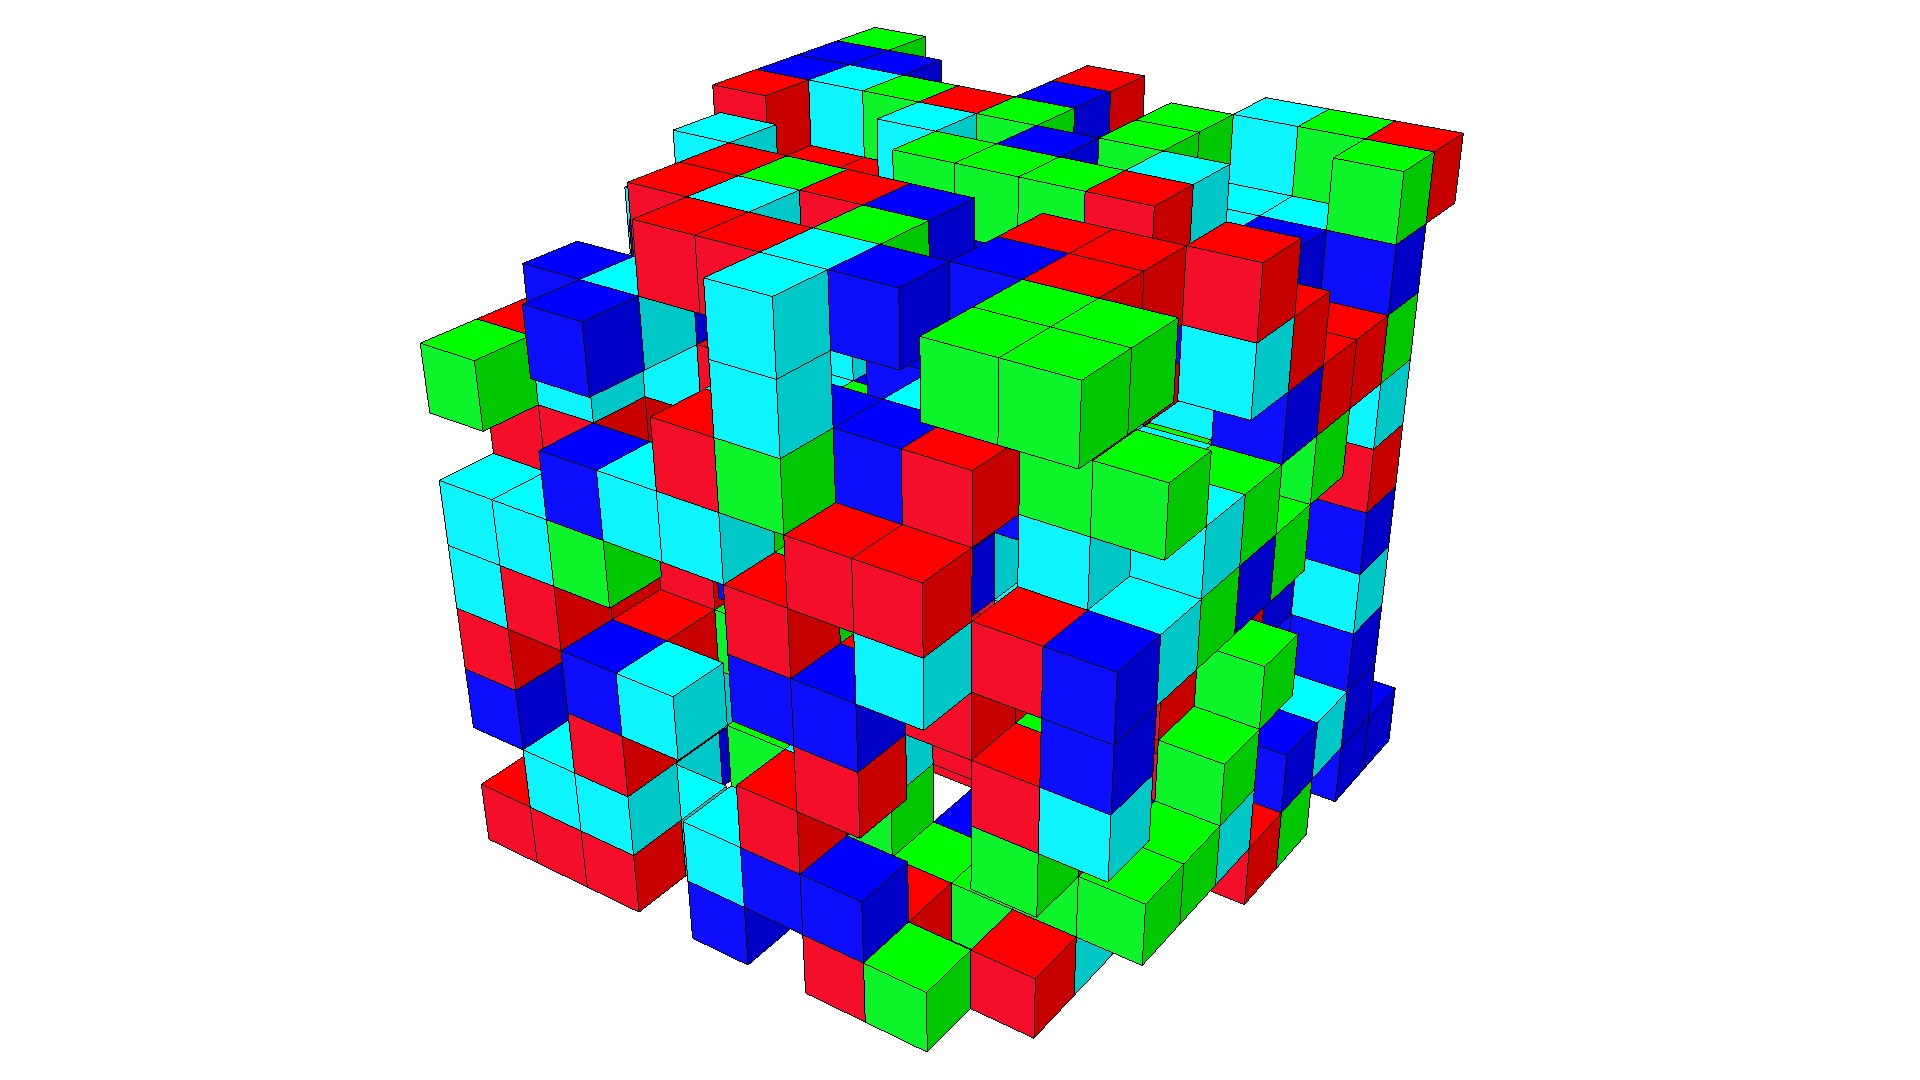
\includegraphics[height=0.2\textheight]{../Figures/Robots/direct.jpg}
\caption{Direct encoding cannot capture the geometrical properties of some problems.}
\label{fig:directRobot}
\end{figure}

In the previous section, indirect and direct random morphology methods were implemented and tested, failing to produce any decent locomotion gaits for the soft structures. Considering how vast is the solution space, random approaches are doomed to fail in a definite number of tries. 

Hence, a more sophisticated method is tested here. Direct encoding genomes coupled with a simple genetic algorithm is a successful approach in evolving robot controllers. As it was previously stated in ch.~\ref{Background}, mutations and crossovers of real value streams, search the space effectively succeeding in difficult optimization problems. GAlib C++ library \cite{wall1996galib}, used for the implementation of this method.

\paragraph*{Representation of the genotype}~\\
As in every direct encoding scheme, genotype can be represented by a stream of bits, which length is equal with the number of the dimensions of the problem. In this case, using 4 materials but also trying to encode the presence of each voxel in the lattice as another dimension of the problem. Analytically, its length can be represented by a stream of length equal with the number of voxels in the lattice times the materials used plus one denoting the presence, descibed by the following equation:
\begin{equation}
\label{lengthDirect}
| Genome | = (l_x \times l_y \times l_z ) \times (1 + |p|)
\end{equation}
, where $l_x, l_y, l_z$ are the dimensions of the lattice space, and $p$ is the palette of materials.
\begin{equation*}
Genome = \underbrace{01010\ldots011011}_\text{Presence}\ \    \underbrace{10101\ldots110011}_{Material_1} \   \ldots\  \underbrace{00011\ldots111110}_{Material_n}
\end{equation*}
The above stream of bit illustrates how a soft-structure in VoxCad environment can be represented. Each of the values of the stream is represented by a value between zero and one, which represented 
in the algorithm by a stream of bits. \emph{Alleles} are continuous numbers in that case, alleles is the definition of each value of the chromosome, which are not shown above due to visualization simplicity. The mapping from the genotype level to the phenotype is straightforward in this case, the first stream of values is used to determine the presence or not for a voxel, while in case of a presence the other $n$ streams are used and the maximum value in specific positions of the streams determine the material is going to be used.

Considering the representation of the genome, as well as the geometrical nature of the problem it self, it is valid to say that we do not expect that direct encoding will capture this major property of the problem (Fig.~\ref{fig:directRobot}).

\section{Generative-Encoded Evolutionary Soft-Robots}

Direct encoding schemes lack the regularity of their designs in the phenotype level leading in morphologies that cannot produce any coordinated locomotion behaviors. Generative-Indirect encoding (CPPN) as it previously explained in detail, serves this function. Producing regularities in the phenotype space, and capturing geometrical properties of the optimization problem, it is expected to produce fine locomotion strategies and morphologies of the soft structures~\cite{cheney2013unshackling}.

\begin{figure}
\centering
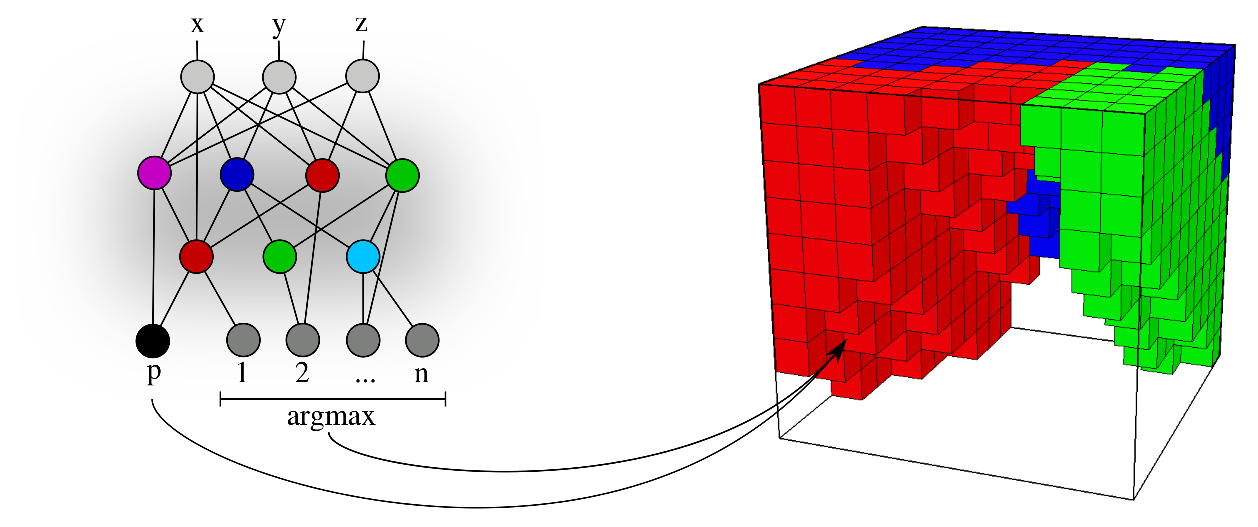
\includegraphics[height=0.2\textheight]{../Figures/Misc/cppnSoftBot2.eps}
\caption{Each genotype is queried for every coordinate inside the lattice, its outputs determine the presence of a voxel and the type of its material.}
\label{fig:cppnDiagram}
\end{figure}


Compositional pattern producing networks are built up by a set of canonical functions which force the outputs of the network to produce repetitive, symmetrical and geometrically interesting patterns. Since, CPPNs must queried for every coordinate of the lattice space, the input nodes of the CPPN were assigned to x,y,z normalized coordinates, following~\cite{cheney2013unshackling}. It should be pointed out here that more inputs could be added to the CPP-network, such as the the distance from the center point of the Cartesian space (simulation lattice) as described in~\cite{stanley2007compositional}, which naturally adds more bias towards symmetrical structures, than CPPNs already do. What is more, creating perfectly symmetrical structures is not much of an interest to show, since CPPNs during evolution, since as shown later in this thesis, it can evolve symmetrical shapes without this symmetrical information input node. Figure~\ref{fig:cppnDiagram}, illustrates the topology of a random CPPN network with the input and output nodes described above. Every connection node between input and output nodes is called the network's \emph{topology} which can be variant and be evolved alongside the weights of the connections in an evolutionary method like NEAT. The shaded part of the network is the part that it is actually the one that describes the genotype and how the phenotype will be structured, while differently colored nodes denote different functions used in them.
Once again, the presence or not of a voxel in a lattice coordinate is determined by a single output of the CPPN called $p$ and the selection of the material out of the palette is again determined by $n$ outputs, the node will the maximum value in the output will determine which of the $n$ materials will be used.


\subsection{How CPPNs can be evolved?}
The evolution of these indirect representations of the phenotypes can be evolved with any method able to evolve artificial neural networks, since they are identical with CPPNs. CPPN-NEAT (first described in Ch.~\ref{Background}), is a method of evolving CPPNs with NEAT evolutionary method, was chosen to evolve those networks as it has proven successful in previous work in the same setting~\cite{cheney2013unshackling}. HyperNEAT \texttt{v4.0 C++} by J. Gauci code (url: \url{https://github.com/MisterTea/HyperNEAT}) was used for the experiments. Algorithm~\ref{evolutionPseudocode}, presents the pseudocode for the evolution under CPPN-NEAT method. In addition, a brief explanation of each function used in the algorithm follows:


\begin{algorithm}[t!]
\caption{CPPN-NEAT evolution}
\label{evolutionPseudocode}
\begin{algorithmic}[1]
\STATE $\mathtt{population} = \varnothing$
\STATE $\mathtt{species} = \varnothing$
\STATE $\mathtt{generation}[0] = \mathbf{initial\_population}()$
\FOR{ $i = 0\   \text{to}\  \mathtt{max\_generation}$}
\STATE $\mathtt{species} = \mathtt{species} \cup \mathbf{speciation}(\mathtt{generation}[i])$
\STATE $\mathbf{evaluation}(\mathtt{generation}[i])$
\STATE $\mathbf{adjust\_fitness}(\mathtt{generation}[i], \mathtt{species})$
\STATE $\mathbf{selection}(\mathtt{generation}[i], \mathtt{species})$
\STATE $\mathtt{generation}[i+1] = \mathbf{reproduction}(\mathtt{generation}[i])$
\STATE $\mathtt{population} = \mathtt{population} \cup \mathtt{generation}[i+1]$
\ENDFOR
\end{algorithmic}
\end{algorithm}

\clearpage % to fit in a page
\begin{framed}
\begin{description}
\item[Initial population]{Before the evolution starts, an initial population must be produced, random genomes (CPPNs) fill up the population.}
\item[Speciation]{ ,takes place and split the population in different species or adds individuals to already existing species in respect to their network's topologies. However, all firstly introduced genomes belong to the same species, due to the identical topology of their CPPNs.}
\item[Evaluation] Once the population is filled with new individuals, these have to be evaluated. Simulation is take place for each of the individuals of the population, whereas each one of them is awarded with a fitness value.
\item[Fitness adjustment]{After all individual are evaluated, each species is assigned a value which is the sum of the fitness values of the individuals belonging to the species divided by the number of the individuals. The way it is been decided how many individuals each of the species will breed is directly determined by the average fitness of each species.}
\item[Selection]{As soon as the number of new individual each species is determined, only the top $20\%$ of the species population will reproduce, the rest population will ``die''.}
\item[Reproduction]{There are three ways, for the selected individual inside each species to reproduce. The first is called \emph{elitism}, meaning that the best of each species will copy itself in the next generation. The next two are \emph{mutation}, which changes the genome of one individual slightly and creates a new genome for the next generation, and \emph{crossover} which is the most natural operator and it uses mixes two parent individuals to create a new genome.}
\end{description}
\end{framed}






\subsection{Novelty search}
Novelty search as first presented in Ch.~\ref{Background}, requires small changes in an evolutionary algorithm. Fitness is replaced by a novelty metric which determines how different is a phenotype's behavior in respect to novel behaviors found before. Sparsity (eq.~\ref{sparsenessEquation}), is used to dermine this measure, whereas every individual is compared not only with the previous novel behaviors but also with the current generation individual behaviors. 



\begin{algorithm}[t!]
\caption{CPPN-NEAT with novelty search}
\label{noveltyPseudocode}
\begin{algorithmic}[1]
\STATE $\mathtt{population} = \varnothing$
\STATE $\mathtt{novel\_inds} = \varnothing$
\STATE $\mathtt{species} = \varnothing$
\STATE $\mathtt{generation}[0] = \mathbf{initial\_population}()$
\FOR{ $i = 0\   \text{to}\  \mathtt{max\_generation}$}
\STATE $\mathtt{species} = \mathtt{species} \cup \mathbf{speciation}(\mathtt{generation}[i])$
\STATE $\mathbf{evaluation}(\mathtt{generation}[i])$
\FORALL {$\mathtt{ind} \in \mathtt{generation}[i]$}
\STATE $\mathtt{novelty} = \mathbf{sparsity}(\mathtt{ind}, (\mathtt{generation}[i] - \mathtt{ind}) \cup \mathtt{novel\_inds})$
\IF {$(\mathtt{novelty} \geq \mathtt{novelty\_{threshold}}\ ||\ \mathtt{novel\_inds} == \varnothing)$}
\STATE $\mathtt{novel\_inds} = \mathtt{novel\_inds} \cup \mathtt{ind}$
\ENDIF
\ENDFOR
\STATE $\mathbf{adjust\_novelty}(\mathtt{generation}[i], \mathtt{species})$
\STATE $\mathbf{selection}(\mathtt{generation}[i], \mathtt{species})$
\STATE $\mathtt{generation}[i+1] = \mathbf{reproduction}(\mathtt{generation}[i])$
\STATE $\mathtt{population} = \mathtt{population} \cup \mathtt{generation}[i+1]$
\ENDFOR
\end{algorithmic}
\end{algorithm}


The algorithmic adjustments are presented in Algorithm~\ref{noveltyPseudocode}, where the pseudocode of novelty search is presented. Instead of just returning a fitness value, function \textbf{evaluation} has as an output the behavior of the individual evaluated, as well as its fitness for comparing purposes. Function \textbf{sparsity}, computes the sparseness of a specific individual's behavior in the behavioral space, calculating the mean distance from the $k$-closest behaviors. Following the evaluation of each individual and the returned point in the behavior space, if the novelty metric is larger than a threshold, this individual will enter the novelty individuals' set. The fitness adjustment of the previous code example is becoming novelty adjustment following the same functionality, selection and reproduction methods are working in the same fashion, whereas they are comparing the novelty of the individual in the place of their fitness.


\subsubsection{Behavior in novelty search}

\begin{table}
\centering
\caption{Behaviors used for novelty metric computation, to evolve morphologies for the soft-robots.}
\label{Behaviors}
    \begin{tabular}{lrcc p{4cm}}
    \toprule
    \textbf{Behavior} &
    \textbf{Sampling} &
    \textbf{DFT} &
    \textbf{Example} &
    \textbf{Description} \\
    \midrule
    \Vcentre{3D-trajectory}    &
    \Vcentre{1 KHz}     &                       &
    \Vcentre{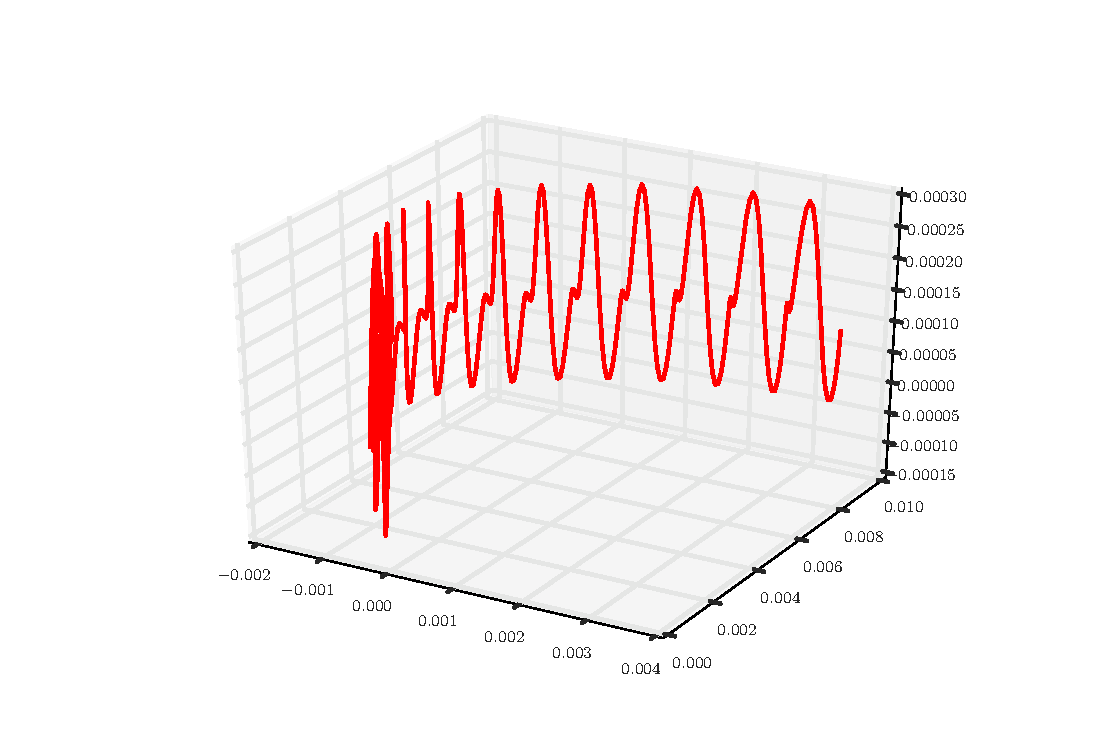
\includegraphics[scale=0.19]{../Figures/Behaviors/3d.pdf}} &
    \vspace{-.85cm}Set of three dimensional sampled points of the robot's center of mass during simulation.  \\
    \Vcentre{2D-trajectory}   &
    \Vcentre{1 KHz}     &                     &
    \Vcentre{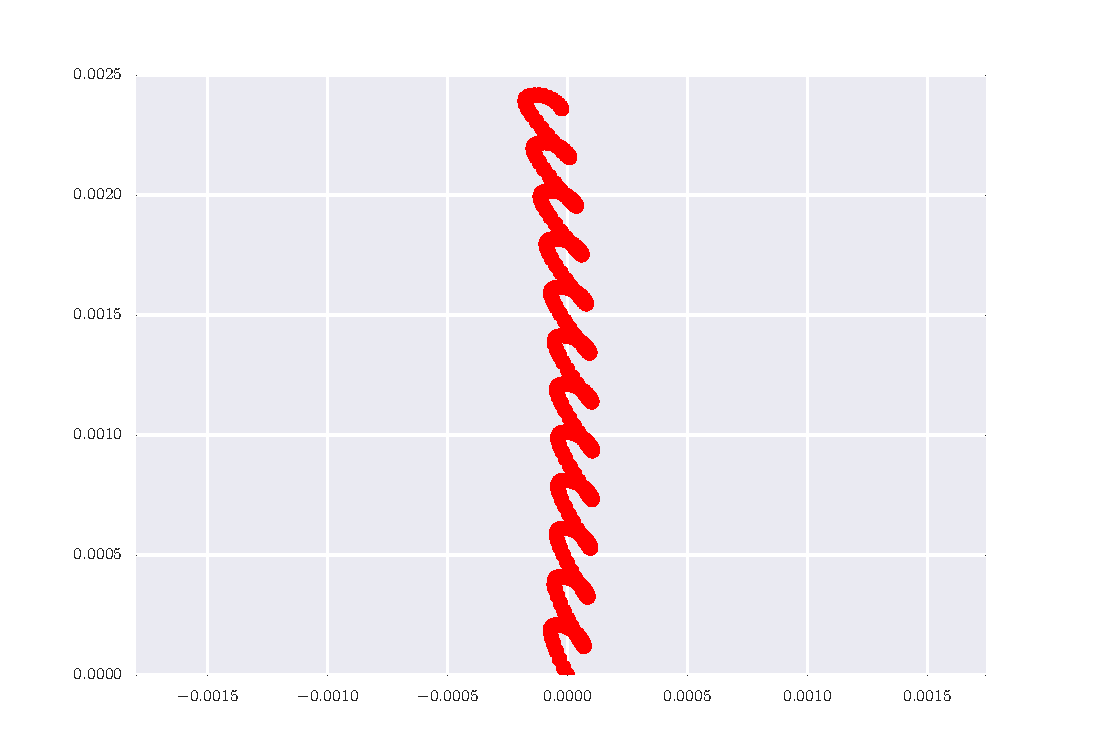
\includegraphics[scale=0.18]{../Figures/Behaviors/2d.pdf}} &
    \vspace{-.85cm}Set of two dimensional ground projection sampled points of the robot's center of mass during simulation.      \\
    \Vcentre{Pace}                 &
    \Vcentre{1 KHz}     &                     &
    \Vcentre{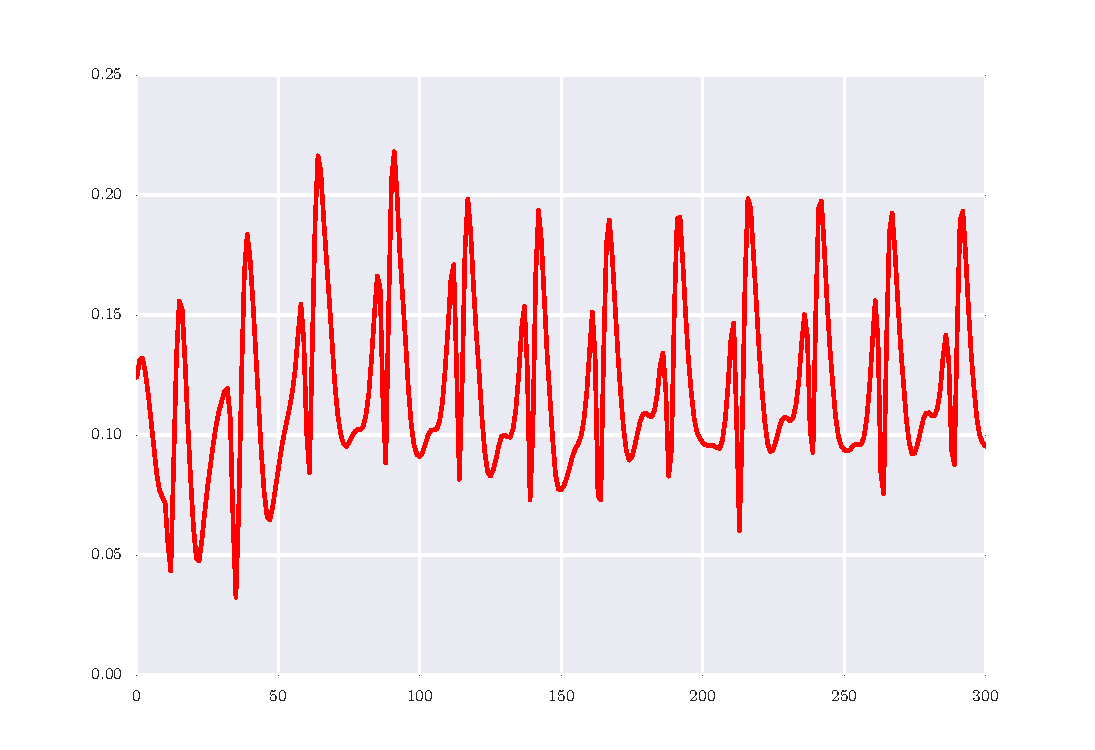
\includegraphics[scale=0.18]{../Figures/Behaviors/pace.pdf}} &
    \vspace{-.85cm}Set of robot's pace sampled values.    \\
    \Vcentre{DFT-Pace}             &
    \Vcentre{100 KHz}   &
    \Vcentre{\checkmark}                &
    \Vcentre{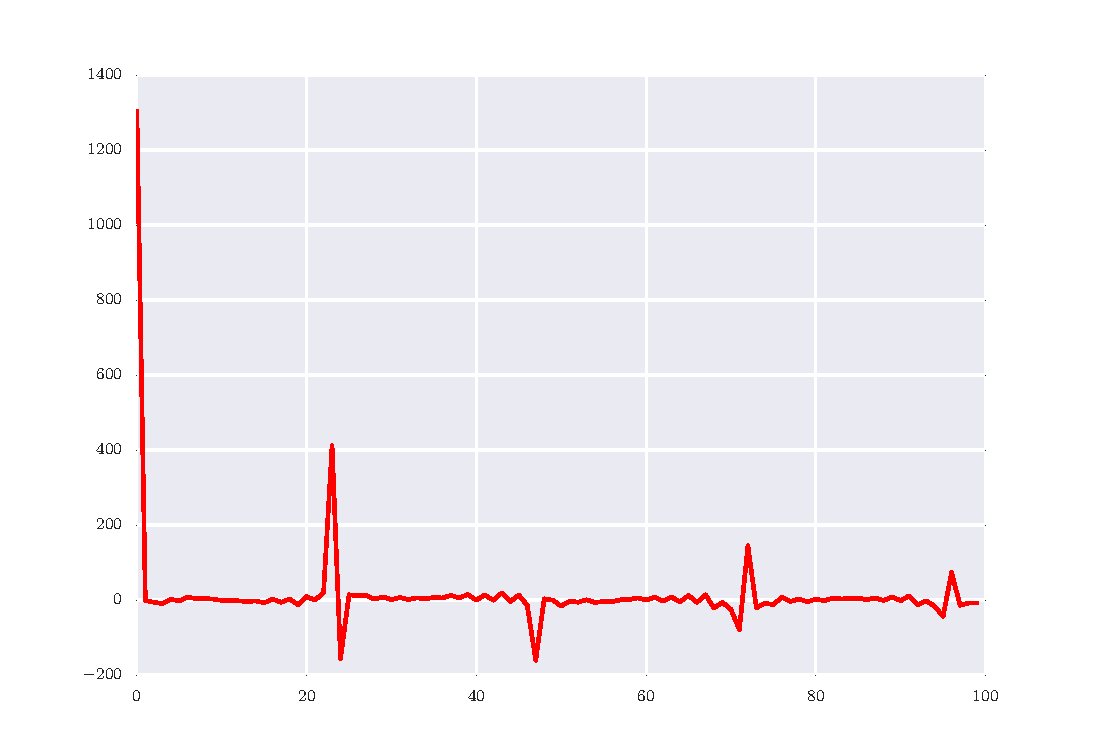
\includegraphics[scale=0.18]{../Figures/Behaviors/pacedft.pdf}} &
    \vspace{-.9cm}Set of the robot's pace sampled values transformed into the frequency space.    \\
    \Vcentre{VTG}                  &
    \Vcentre{1 KHz}     &                     &
    \Vcentre{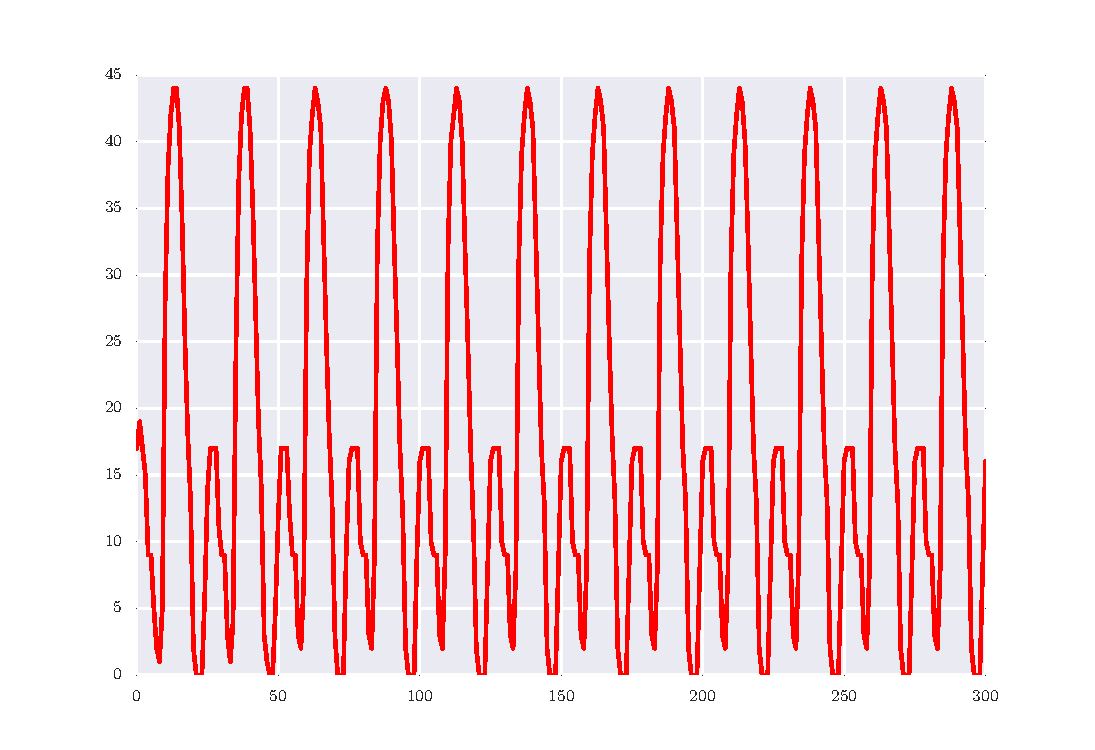
\includegraphics[scale=0.18]{../Figures/Behaviors/vtg.pdf}} &
    \vspace{-.85cm}  Voxels touching the ground in each sampling time.  \\
    \Vcentre{DFT-VTG}              &
    \Vcentre{100 KHz}   &
    \Vcentre{\checkmark}              &
    \Vcentre{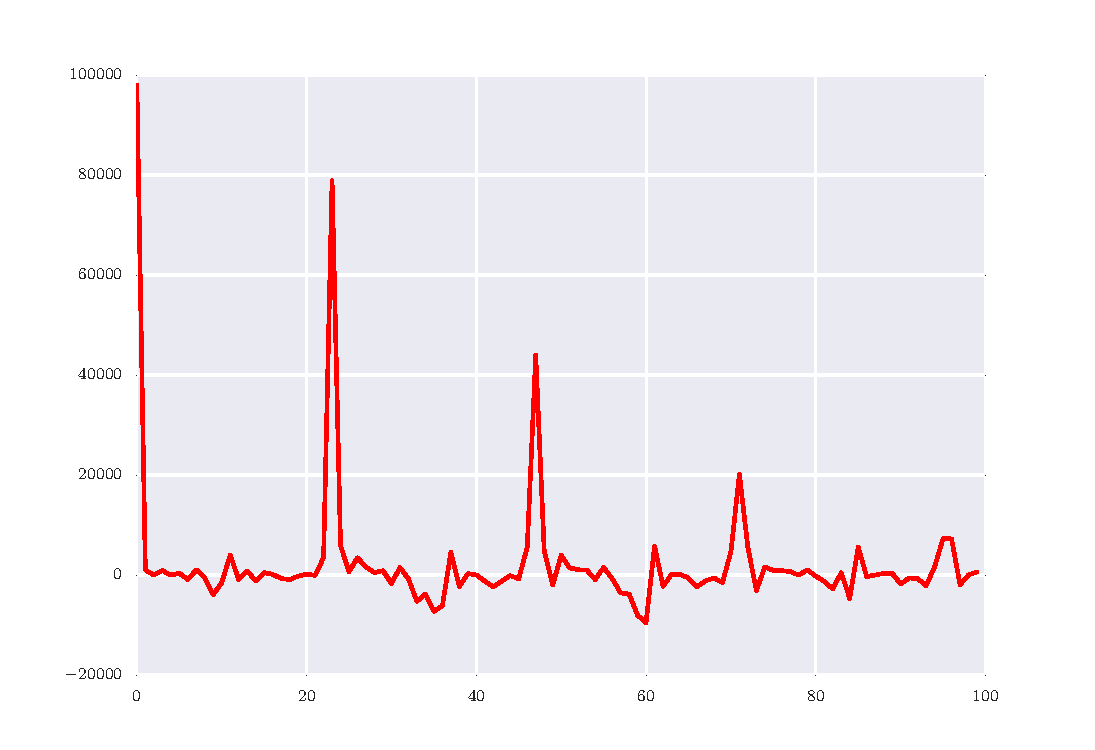
\includegraphics[scale=0.18]{../Figures/Behaviors/vtgdft.pdf}} &
    \vspace{-.85cm} Voxels touching the ground transformed into the frequency space.   \\
    \Vcentre{Pressure}             &
    \Vcentre{1 KHz}     &                     &
    \Vcentre{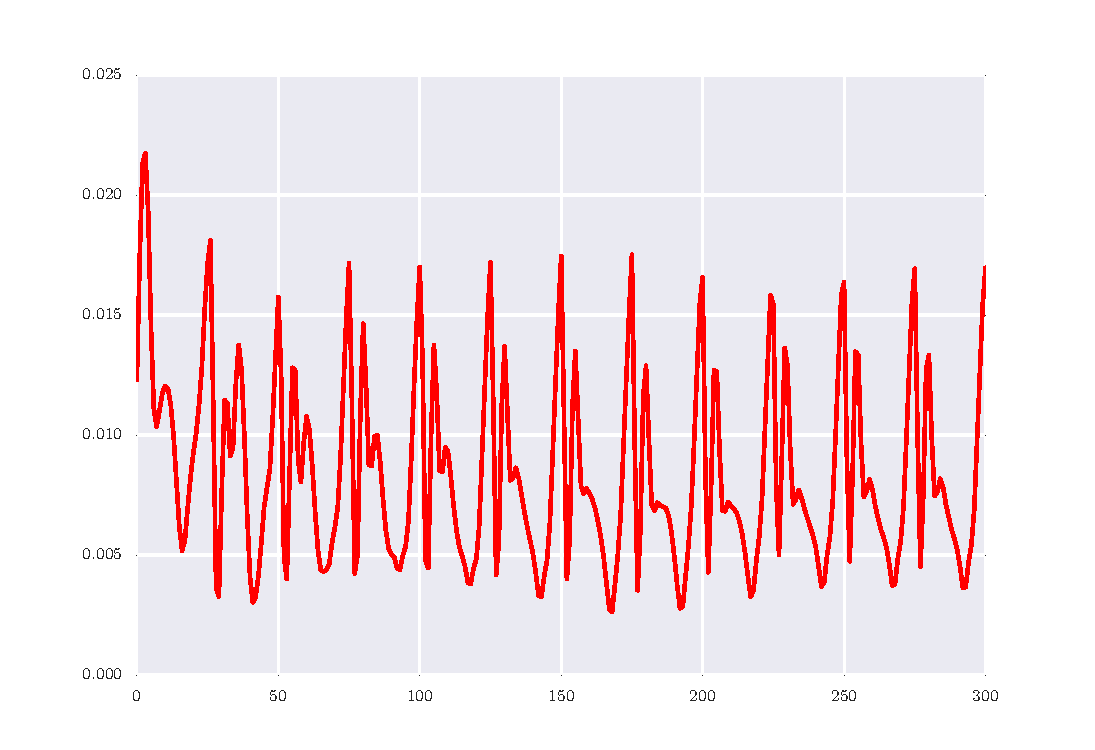
\includegraphics[scale=0.18]{../Figures/Behaviors/pr.pdf}} &
    \vspace{-.85cm}Maximum pressure among the connected voxels.  \\
    \Vcentre{DFT-Pressure}         &
    \Vcentre{100 KHz}   &
    \Vcentre{\checkmark}                &
    \Vcentre{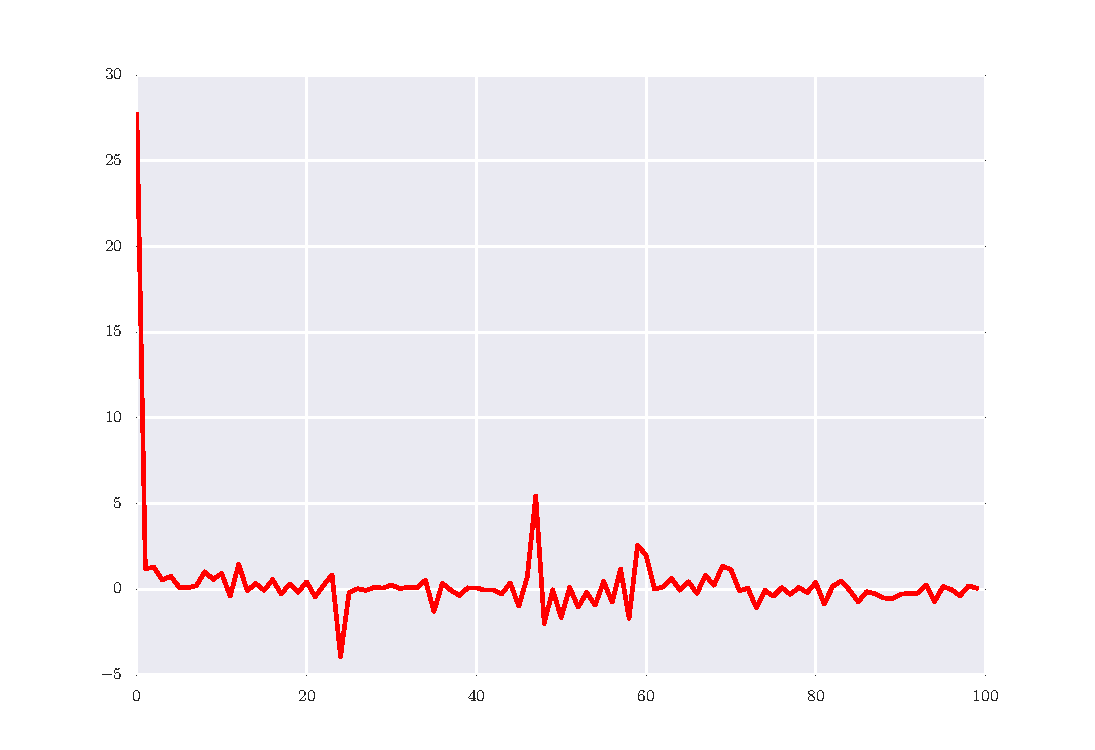
\includegraphics[scale=0.18]{../Figures/Behaviors/prdft.pdf}} &
    \vspace{-.85cm}Maximum pressure among the connections transformed into the frequency space.    \\
    \Vcentre{KE}                   &
    \Vcentre{1 KHz}     &                     &
    \Vcentre{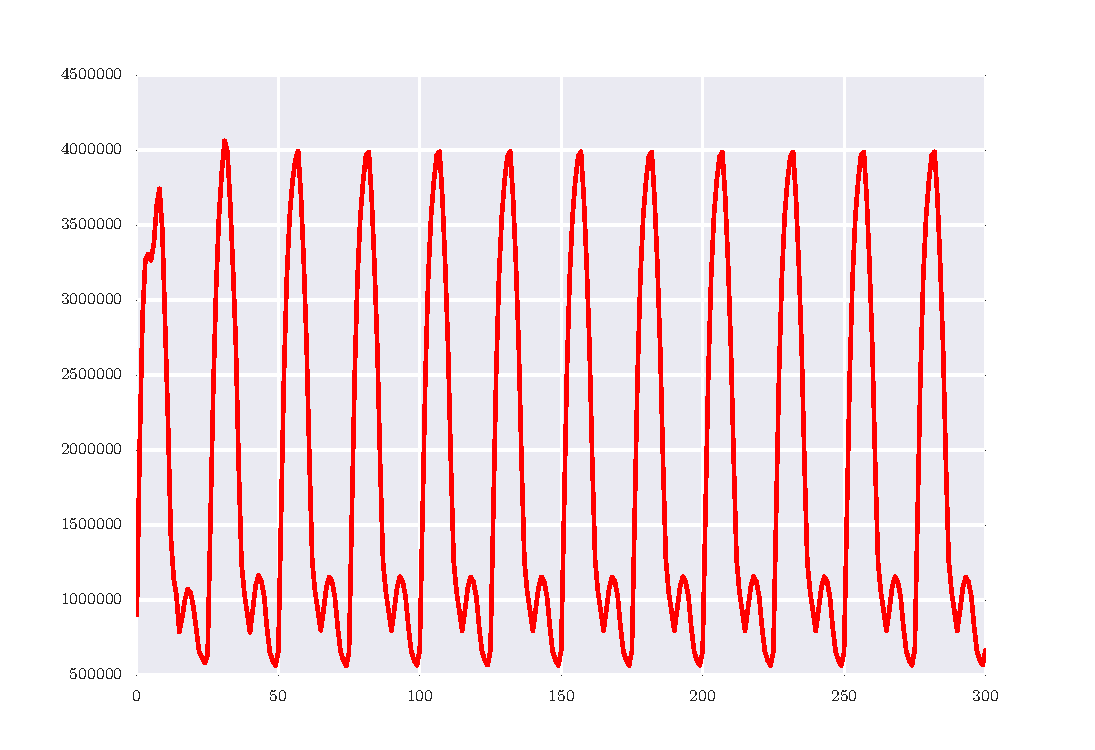
\includegraphics[scale=0.18]{../Figures/Behaviors/ke.pdf}} &
    \vspace{-.85cm}Maximum kinetic energy of voxels.    \\
    \Vcentre{DFT-KE}               &
    \Vcentre{100 KHz}   &
    \Vcentre{\checkmark}                &
    \Vcentre{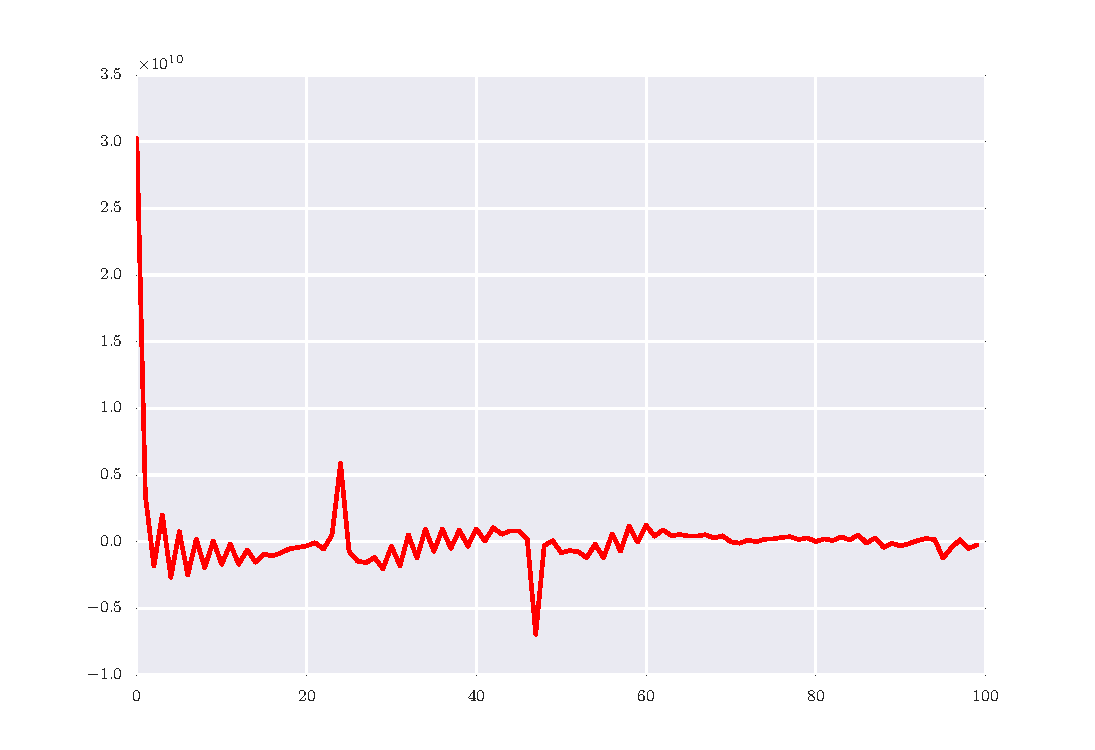
\includegraphics[scale=0.18]{../Figures/Behaviors/kedft.pdf}}  &
    \vspace{-.85cm}Maximum kinetic energy of voxels transformed into the frequency space.    \\
    \bottomrule
    \end{tabular}
\end{table}

In the interest of novelty to be defined, behaviors should be defined that make sense in our problem setting. Trying to optimize locomotion strategies of soft-robots under variant environment in fitness-based methods, a good measure is the displacement under a limited time-span. On the contrary, novelty search is in a need of a behavior metric that encodes these fitness attributes inside. Novelty search forces the evolution to try new behaviors, if the objective cannot be encoded in the behavior, the search then novelty search will become random. As an example, the number of voxels a soft robot has is not a well-founded behavior metric, since the search will reward new structures with different number of voxels from previous ones, there will be no exploration in a metric that affects the actual target of the evolution which is to produce and evolve good locomotion strategies. Table~\ref{Behaviors}, presents all behaviors used for novelty metric computation, with the sampling rates of the recorded values during the simulation and a description. 

All these behaviors designed having in mind that enough information about the locomotion success must be encoded into the behavior's recorded signal. Trajectories (2D and 3D), incorporate all the needed information, such as speed, displacement, locomotion strategy. To avert from same trajectories in all possible directions, trajectories are normalized, meaning that their starting coordinate in both cases (2D and 3D) is always the start of the axes, and their all coordinates of the trajectory are rotated so their center of mass coordinate is normalized to meet a certain angle. Computing the difference of two trajectories, the Euclidean distances of all coordinates of the one trajectory are computer in respect to coordinates at the same sampling time.

Pace is also a very informative behavior metric as it directly measures the speed of the robot. Voxels touching the ground can also produce information about the locomotion strategy but not enough about the actual performance speed-wise. Hopping robots that move fast can have same behaviors with hopping robots with zero speed. Maximum pressure among the voxels' connection is one more behavior metric, pressure is expected to become higher as structures move faster and interactions with the ground eventually being harder. Finally, maximum kinetic energy is a different behavior that straightly determines the displacement of the voxels in the structure. For all behaviors but trajectories, the Fourier profile of their signal can also be used as a behavior signature of the individuals, which can also eliminate shifts of signals in time-axis. To compute the difference of over two signals a straightforward method is chosen. Subtracting the one signal from the other taking the absolute differences and sum them up to compute one signle value that describes how variant the two signals are. Furthermore, for the Fourier transformations of these signals, the first twenty coefficients are compared, the absolute sum difference again determines the difference.